\section{Interferometric Diagnostics and the Abel Transform}

The propagation code produces a three dimensional map of the free electron density, the self-trapped exciton density, and the intensity, but none of these quantities can be measured directly inside a bulk sample. What can be measured is the phase shift accumulated by a probe beam that crosses the excited region, using a Nomarski interferometer. This section derives how that phase shift relates to the refractive index change predicted by the simulation, and describes how \texttt{unified\_filament\_slider\_v3.py} implements both directions of this link, from a measured interferogram back to a refractive index profile, and from a simulated refractive index profile forward to a predicted interferogram. The physical setup and the mathematics of the Abel transform below are identical whether the excited medium is air or fused silica, only the propagation equation that produces the refractive index change differs, and that equation was already given in Section~11 for $\mathrm{SiO}_2$.

\subsection{Two-Plane-Wave Interferometry}

The Nomarski interferometer can be understood as a configuration that allows retrieval of phase information about a medium under investigation. We derive the fundamental equations governing the interference pattern produced by two plane waves with different propagation directions.

\subsubsection{Field Configuration and Wave Vectors}

Consider two plane waves propagating in the same medium with refractive index $\eta_i$:
\begin{equation}
E_1 = \underline{E_0} \, e^{i(\vec{k}_1 \cdot \vec{r} - \omega t)}
\end{equation}
\begin{equation}
E_2 = \underline{E_0} \, e^{i(\vec{k}_2 \cdot \vec{r} - \omega t)}
\end{equation}
where the wave vectors are defined as:
\begin{equation}
\vec{k}_1 = \frac{2\pi}{\lambda}\eta_i \begin{pmatrix}\sin{\theta}\\0\\\cos{\theta}\end{pmatrix} = k \begin{pmatrix}\sin{\theta}\\0\\\cos{\theta}\end{pmatrix}, \qquad
\vec{k}_2 = k \begin{pmatrix}-\sin{\theta}\\0\\\cos{\theta}\end{pmatrix}
\end{equation}
These two plane waves propagate symmetrically with respect to the normal axis, making an angle $2\theta$ with each other. To account for an arbitrary orientation of the fringes around the $z$ axis, we introduce a rotation of angle $\phi$, which turns the wave vectors into $k(\cos\phi\sin\theta,\sin\phi\sin\theta,\cos\theta)$ and its mirror image.

\subsubsection{Intensity Distribution and Fringe Spacing}

Setting the observation screen at $z=0$, the intensity is:
\begin{equation}
I(x,y) = I_1 + I_2 + \sqrt{I_1I_2} \cos\big((\vec{k}_1 - \vec{k}_2) \cdot \vec{r}\big)
\end{equation}
For equal amplitudes and after computing the phase difference $(\vec{k}_1-\vec{k}_2)\cdot\vec{r} = 2k\sin\theta(x\cos\phi+y\sin\phi)$, this becomes:
\begin{equation}
\boxed{I(x,y) = 2I_0(x,y)\left[1 + \cos\big(2\pi \nu_0(x\cos{\phi}+y\sin{\phi}\big)\right]}, \qquad \nu_0 = \frac{2\sin\theta}{\lambda}
\end{equation}
where $\nu_0$ is the spatial-carrier frequency of the fringes, set purely by the crossing angle $2\theta$ of the two interfering beams, and independent of anything happening inside the medium.

\begin{figure}[h!]
    \centering
    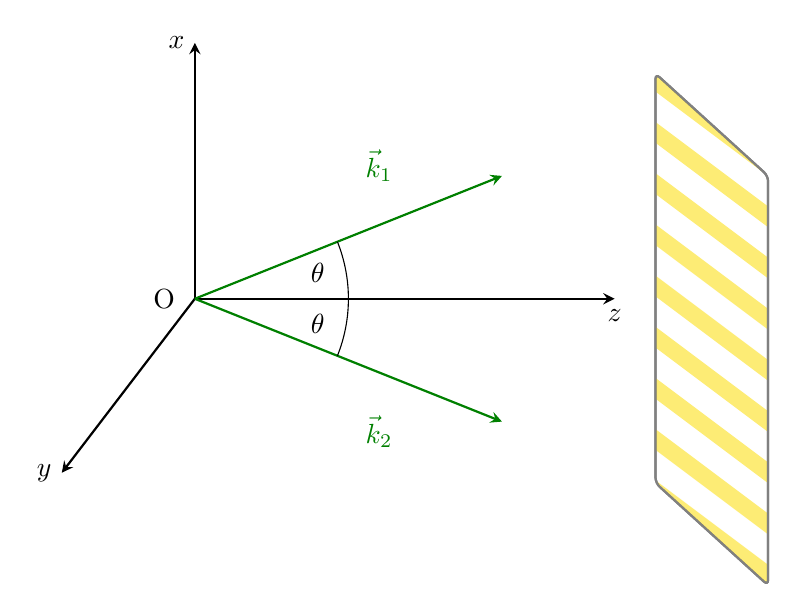
\begin{tikzpicture}[scale=1.3]
        \draw[-stealth, thick] (0,0) -- (0,2.5) node[left] {$x$};
        \draw[-stealth, thick] (0,0) -- (-1.3,-1.7) node[left] {$y$};
        \draw[-stealth, thick] (0,0) -- (4.1,0) node[below] {$z$};
        \node[left] at (-0.1, 0) {O};
        \def\screen{
            (4.5, 2.2) -- (5.6, 1.2) -- (5.6, -2.8) -- (4.5, -1.8) -- cycle
        }
        \draw[gray, thick, fill=white, rounded corners=2pt] \screen;
        \begin{scope}
            \clip[rounded corners=2pt] \screen;
            \foreach \i in {-4,-3.5,...,4} {
                \draw[yellow!80!orange, line width=6pt, opacity=0.55] (4, \i) -- (6, \i-1.5);
            }
        \end{scope}
        \draw[gray, thick, rounded corners=2pt] \screen;
        \draw[-stealth, thick, green!50!black] (0,0) -- (3, 1.2);
        \node[green!50!black] at (1.8, 1.3) {$\vec{k}_1$};
        \draw[-stealth, thick, green!50!black] (0,0) -- (3, -1.2);
        \node[green!50!black] at (1.8, -1.3) {$\vec{k}_2$};
        \draw (1.5,0) arc (0:21.8:1.5);
        \node at (1.2, 0.25) {$\theta$};
        \draw (1.5,0) arc (0:-21.8:1.5);
        \node at (1.2, -0.25) {$\theta$};
    \end{tikzpicture}
    \caption{Interference of two plane waves propagating symmetrically with an angle $2\theta$, creating an interference pattern on the screen (shown for $\phi = 0$).}
    \label{fig:interference}
\end{figure}

\subsection{Phase and Amplitude Extraction via Fourier Analysis}

Nomarski interferograms read $I(x,y) = a(x,y) + b(x,y)\cos\!\big[2\pi\nu_0 x + \varphi(x,y)\big]$, where $a(x,y)$ is the background term, $b(x,y)$ the amplitude modulation term, and $\varphi(x,y)$ the phase of interest, related to the line integrated electron density by $\varphi(x,y) \propto \int n_e(x,y,z)\,\mathrm{d}z$. In conventional contour-fringe interferometry, obtained when $\nu_0=0$, the intensity reads $I = a + b\cos\varphi$, in which $a$, $b$, and $\varphi$ are mixed, which limits accuracy, and the parity of the cosine prevents determining the sign of $\varphi$.

The Takeda method~\cite{takeda1982fourier} overcomes both limitations through spatial homodyne demodulation. As in classical heterodyne detection, the signal of interest is carried by an oscillating reference, here the spatial carrier $\nu_0$ generated by the tilted incidence angle of the interferometer arms. Writing the cosine with Euler's formula gives $I(x,y) = a(x,y) + c(x,y)e^{i2\pi\nu_0 x} + c^*(x,y)e^{-i2\pi\nu_0 x}$ with $c(x,y) = \tfrac{1}{2}b(x,y)e^{i\varphi(x,y)}$. Bandpass filtering around $+\nu_0$ in the Fourier plane isolates the sideband carrying $c(x,y)$ alone, from which $b$ and $\varphi$ are recovered respectively as the modulus and the argument.

This linear separation also improves sensitivity to weak phase variations. Contour interferometry responds quadratically to a small phase, $\Delta I_{contour} \approx \tfrac{b}{2}\varphi^2$, because small variations sit near the extremum of a cosine, whereas the Takeda method responds linearly, $\Delta I_{Takeda} \approx -b\sin(2\pi\nu_0 x)\,\varphi$, which is what gives it sub-wavelength phase sensitivity~\cite{takeda1982fourier}. Applied to a reference interferogram (no plasma or no excitation) and a measurement interferogram, the ratio of the two filtered and inverse transformed signals cancels the carrier and any residual optical misalignment:
\begin{equation}
z(x,y) \equiv \frac{I_{\text{meas,filt}}(x,y)}{I_{\text{ref,filt}}(x,y)} = \frac{b_2(x,y)}{b_1(x,y)}\,e^{i\varphi(x,y)}, \qquad
\boxed{\varphi(x,y) = \operatorname{atan2}\big(\Im{(z)},\Re{(z)}\big)}
\end{equation}

\subsection{Resolution Limits}

Two independent limits set the finest feature that can be resolved. The Nyquist limit comes from the pixelated sensor. The shortest oscillation observable without aliasing must span at least two pixels, giving $\nu_N = 1/(2\Delta x)$ with $\Delta x$ the pixel size. The optical limit comes from diffraction at the sample itself. A feature of size $d$ diffracts light at an angle $\sin\theta = \lambda/d$, as illustrated in Figure~\ref{fig:diffraction_slit}, and this diffracted light is only collected by the imaging lens if $\sin\theta \le NA$.

\begin{figure}[h!]
    \centering
    \begin{tikzpicture}[scale=0.62]
        \foreach \x in {-4, -3.2, -2.4, -1.6, -0.8} {
            \draw[decorate, decoration={snake, amplitude=0.35mm, segment length=2.5mm}, thin] (\x, 2.5) -- (\x, -2.5);
        }
        \draw[thick, fill=white, line join=round] (-3.6, -0.5) -- (-2.0, -0.5) -- (-2.0, -0.9) -- (-1.0, 0) -- (-2.0, 0.9) -- (-2.0, 0.5) -- (-3.6, 0.5) -- cycle;
        \fill[black!90] (0, 1.2) rectangle (0.35, 4);
        \fill[black!90] (0, -1.2) rectangle (0.35, -4);
        \draw[<->, >=stealth, thick] (-0.3, 0.2) -- (-0.3, -0.2) node[midway, left] {$d$};
        \draw[thin, gray] (-0.6, 1.2) -- (0, 1.2);
        \draw[thin, gray] (-0.6, -1.2) -- (0, -1.2);
        \draw[densely dashed, thick] (0, 1.2) -- (0, -1.2);
        \def\angleDev{26}
        \foreach \y in {1.0, 0.75, 0.5, 0.25, 0, -0.25, -0.5, -0.75, -1.0} {
            \draw[-{Stealth[length=2.5mm, width=1.5mm]}, blue!70!black, thin] (0, \y) -- ++(\angleDev:7.5);
            \draw[-{Stealth[length=2.5mm, width=1.5mm]}, black, thin] (0, \y) -- ++(0:7.5);
            \draw[-{Stealth[length=2.5mm, width=1.5mm]}, blue!70!black, thin] (0, \y) -- ++(-\angleDev:7.5);
        }
        \draw[thick, red!80!black] (4,0) arc (0:\angleDev:4) node[midway, right, xshift=2pt] {$\theta$};
        \node[right] at (7.5, {7.5*tan(\angleDev)}) {\small 1st order};
        \node[right] at (7.5, 0) {\small 0th order};
        \node[right] at (7.5, {-7.5*tan(\angleDev)}) {\small -1st order};
    \end{tikzpicture}
    \caption{A feature of size $d$ diffracts the probe beam into orders separated by $\sin\theta=\lambda/d$. Only orders within the lens acceptance angle are collected.}
    \label{fig:diffraction_slit}
\end{figure}

Inverting the problem gives the smallest resolvable feature for a lens of numerical aperture $NA=\sin\alpha$ in a coherent on axis configuration, $R_0=\lambda/NA$, shown in Figure~\ref{fig:diffraction_NA}. After magnification by the imaging system, the highest spatial frequency actually delivered to the sensor is $\nu_{max} = NA/(M_{tot}\lambda)$, and the digital sampling must satisfy $\nu_N \ge \nu_{max}$ for the optical resolution to be preserved rather than lost to undersampling.

\begin{figure}[h!]
    \centering
    \begin{tikzpicture}[scale=0.62]
        \foreach \x in {-5.2, -4.4, -3.6, -2.8, -2.0} {
            \draw[decorate, decoration={snake, amplitude=0.35mm, segment length=2.5mm}, thin] (\x, 2.5) -- (\x, -2.5);
        }
        \draw[<->, >=stealth, thick] (-3.6, 2.2) -- (-2.8, 2.2) node[midway, above] {$\lambda$};
        \draw[thick, fill=white, line join=round] (-4.0, -0.5) -- (-2.2, -0.5) -- (-2.2, -0.9) -- (-1.2, 0) -- (-2.2, 0.9) -- (-2.2, 0.5) -- (-4.0, 0.5) -- cycle;
        \fill[black!90] (0, 1.2) rectangle (0.35, 4);
        \fill[black!90] (0, -1.2) rectangle (0.35, -4);
        \draw[thin, gray] (-1.0, 1.2) -- (0, 1.2);
        \draw[thin, gray] (-1.0, -1.2) -- (0, -1.2);
        \draw[densely dashed, thick] (0, 1.2) -- (0, -1.2);
        \draw[<->, >=stealth, thick, orange] (-0.3, 0.2) -- (-0.3, -0.2) node[midway, left=4pt] {$R_0$};
        \draw[<->, >=stealth, thick] (-0.3, 1.1) -- (-0.3, 0.3) node[midway, left=4pt] {$d$};
        \def\angleDev{26}
        \foreach \y in {0} {
            \draw[-{Stealth[length=2.5mm, width=1.5mm]}, blue!70!black, thick] (0, \y) -- ++(\angleDev:8.5);
            \draw[-{Stealth[length=2.5mm, width=1.5mm]}, black, thick] (0, \y) -- ++(0:8.5);
            \draw[-{Stealth[length=2.5mm, width=1.5mm]}, blue!70!black, thick] (0, \y) -- ++(-\angleDev:8.5);
        }
        \def\lensX{6.5}
        \def\lensY{4.0}
        \draw[thick, fill=cyan!10, opacity=0.8] (\lensX, \lensY) to[bend left=15] (\lensX, -\lensY) to[bend left=15] cycle;
        \draw[dash dot, thin, gray] (\lensX, \lensY+0.5) -- (\lensX, -\lensY-0.5);
        \draw[densely dashed, thick, orange!90!black] (0,0) -- (\lensX, \lensY);
        \draw[densely dashed, thick, orange!90!black] (0,0) -- (\lensX, -\lensY);
        \pgfmathsetmacro{\angleAlpha}{atan(\lensY/\lensX)}
        \draw[thick, orange!90!black] (4.5,0) arc (0:\angleAlpha:4.5) node[midway, right, xshift=2pt, yshift=4pt] {$\alpha$};
        \node[orange!90!black, right] at (\lensX-4.5, \lensY-0.5) {$\mathrm{NA} = \sin \alpha = \frac{\lambda}{R_0}$};
        \draw[thick, red!80!black] (2,0) arc (0:\angleDev:2) node[midway, right, xshift=2pt] {$\theta \left( \sin\theta = \frac{\lambda}{d} \right)$};
        \node[right] at (8, {7.8*tan(\angleDev)}) {\small 1st order};
        \node[right] at (8.5, 0) {\small 0th order};
        \node[right] at (8, {-7.8*tan(\angleDev)}) {\small -1st order};
    \end{tikzpicture}
    \caption{Smallest resolvable feature $R_0=\lambda/NA$ for a lens of numerical aperture $NA=\sin\alpha$, obtained by requiring the first diffraction order to fall within the acceptance cone.}
    \label{fig:diffraction_NA}
\end{figure}

\authornote{The two remaining subsections of the source document, on off-axis digital holography bandwidth and the DFT based reconstruction method, were left unfinished (marked \emph{to be edited} in the original file). I have not included them here since I cannot complete the derivation without knowing what you intended for the carrier bandwidth argument. Send me the intended argument or your notes and I will finish this part.}

\subsection{The Abel Transform}

Consider a probe beam crossing the excited cylindrically symmetric region along $y$, at fixed $x$ and $z$. The accumulated phase relative to a beam that has not crossed the excited region is:
\begin{equation}
\phi(x,z) = 2\left(\frac{2\pi}{\lambda_L}\right)\int_0^{\infty}[\eta(r,z) - 1] \, dy, \qquad r = \sqrt{x^2+y^2}
\end{equation}
Using the substitution $y = \sqrt{r^2 - x^2}$, this line integral becomes the forward Abel transform of the refractive index deviation $f(r) \equiv \eta(r,z)-1$:
\begin{equation}
\boxed{F(x) = 2\int_x^{\infty} \frac{f(r) \, r}{\sqrt{r^2 - x^2}} \, dr}, \qquad F(x) \equiv \frac{\lambda_L}{4\pi}\phi(x,z)
\end{equation}
This is consistent with equation (4) of reference~\cite{gonzalez2012plasma}. The Abel transform can be inverted analytically. Applying the operator $\int_\rho^\infty x\,dx/\sqrt{x^2-\rho^2}$ to both sides and using the identity $\int_\rho^r x\,dx/\sqrt{(r^2-x^2)(x^2-\rho^2)} = \pi/2$ gives, after differentiating with respect to $\rho$:
\begin{equation}
\boxed{f(\rho) = -\frac{1}{\pi} \int_{\rho}^{\infty} \frac{dF(x)/dx}{\sqrt{x^2 - \rho^2}} \, dx}
\qquad\Longrightarrow\qquad
\boxed{\eta(r,z) = 1 - \frac{1}{\pi}\left(\frac{\lambda_L}{2\pi}\right)\int_r^{\infty} \frac{d\phi(x,z)/dx}{\sqrt{x^2 - r^2}} \, dx}
\end{equation}

The Abel transform is also a special case of the more general Radon transform, which describes the line integral of a function along an arbitrary ray at angle $\theta$ and impact parameter $\rho$. For a rotationally symmetric function $f(r)$, the projection is the same at every angle, and choosing $\theta=0$ turns the Radon integral into $\mathcal{R}[f](\rho) = 2\int_\rho^\infty f(r)\,r\,dr/\sqrt{r^2-\rho^2}$, exactly the forward Abel transform above. This equivalence is what justifies treating the interferometric phase, a line integrated quantity, as a projection that can be inverted whenever cylindrical symmetry holds.

\subsection{Numerical Inversion by the Trapezoidal Rule}

To invert the Abel transform numerically, the integral is approximated by summing trapezoidal areas $A_k \approx \tfrac12(x_{k+1}-x_k)[g(x_{k+1})+g(x_k)]$ over the integrand $g(x_k,r_i) = \big[dF(x)/dx\big]_{x=x_k}/\sqrt{x_k^2-r_i^2}$. The derivative is itself approximated by a forward difference, $dF/dx|_{x_k} \approx [F(x_{k+1})-F(x_k)]/\Delta x$, and the integration starts one pixel away from $x=r_i$ to avoid the mathematical singularity there. Substituting the forward difference into the trapezoidal sum, the step size $\Delta x$ cancels exactly, leaving:
\begin{equation}
\boxed{f(r_i) = -\frac{1}{2\pi}\sum_{k=i+1}^{N-2} \left[ \frac{F(x_{k+2}) - F(x_{k+1})}{\sqrt{x_{k+1}^2 - r_i^2}} + \frac{F(x_{k+1}) - F(x_k)}{\sqrt{x_k^2 - r_i^2}} \right]}
\end{equation}
directly implementable without ever storing $\Delta x$ as a separate factor.

\begin{figure}[h!]
    \centering
    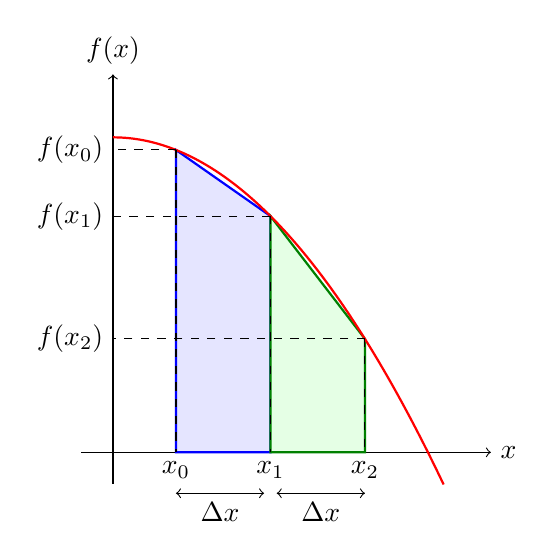
\begin{tikzpicture}[scale=4]
        \draw[->] (-0.1,0) -- (1.2,0) node[right] {$x$};
        \draw[->] (0,-0.1) -- (0,1.2) node[above] {$f(x)$};
        \def\xa{0.2}
        \def\xb{0.5}
        \def\xc{0.8}
        \def\fa{0.96}
        \def\fb{0.75}
        \def\fc{0.36}
        \fill[blue!10] (\xa,0) -- (\xa,\fa) -- (\xb,\fb) -- (\xb,0) -- cycle;
        \draw[blue, thick] (\xa,0) -- (\xa,\fa) -- (\xb,\fb) -- (\xb,0) -- cycle;
        \fill[green!10] (\xb,0) -- (\xb,\fb) -- (\xc,\fc) -- (\xc,0) -- cycle;
        \draw[green!50!black, thick] (\xb,0) -- (\xb,\fb) -- (\xc,\fc) -- (\xc,0) -- cycle;
        \draw[thick, red, domain=0:1.05, samples=100] plot (\x, {-\x*\x + 1});
        \draw[dashed] (\xa, \fa) -- (\xa, 0) node[below] {$x_0$};
        \draw[dashed] (\xb, \fb) -- (\xb, 0) node[below] {$x_1$};
        \draw[dashed] (\xc, \fc) -- (\xc, 0) node[below] {$x_2$};
        \draw[dashed] (\xa, \fa) -- (0, \fa) node[left] {$f(x_0)$};
        \draw[dashed] (\xb, \fb) -- (0, \fb) node[left] {$f(x_1)$};
        \draw[dashed] (\xc, \fc) -- (0, \fc) node[left] {$f(x_2)$};
        \draw[<->] (\xa, -0.13) -- node[below] {$\Delta x$} (\xb-0.02, -0.13);
        \draw[<->] (\xb+0.02, -0.13) -- node[below] {$\Delta x$} (\xc, -0.13);
    \end{tikzpicture}
    \caption{Illustration of the trapezoidal rule for numerical integration. The integral under the curve is approximated as a sum of trapezoidal areas.}
    \label{fig:trapezoidal}
\end{figure}

\subsection{Connecting the Simulation to the Diagnostic: \texttt{unified\_filament\_slider\_v3.py}}

The script \texttt{unified\_filament\_slider\_v3.py} implements both directions of the link between the simulation and a real interferometric measurement, so that the two can be compared directly.

On the experimental side, \texttt{find\_1storder\_peak} locates the side band of a raw interferogram in Fourier space by masking out the central DC region and searching for the strongest remaining peak, implementing the Takeda demodulation step described above. \texttt{reconstruct} then crops a disk of radius set by the numerical aperture around that peak and inverse transforms it back to real space, giving the complex field $c(x,y)$ from which the phase is extracted. \texttt{fit\_plane\_from\_mask}, applied over user selected background regions through \texttt{baseline\_rects\_to\_mask}, removes any residual linear phase tilt from small optical misalignments that the reference division does not fully cancel, exactly the correction motivated at the end of the phase retrieval derivation above. \texttt{preprocess\_side\_full} chains these steps into the full pipeline from a raw pair of interferograms, signal and reference, to a clean two dimensional phase map.

On the simulation side, \texttt{build\_abel\_matrix} discretizes the forward Abel transform directly as a matrix acting on the non uniform radial grid produced by the QDHT, using the exact shell integral of $r/\sqrt{r^2-x^2}$ over each radial bin rather than a naive trapezoidal sum on that grid, so that the same physical relation $F(x)=2\int_x^\infty f(r)r\,dr/\sqrt{r^2-x^2}$ used above for the inversion is applied here in the forward direction. \texttt{abel\_phase\_2d} assembles the total refractive index change $\Delta n$ from every channel the propagation code tracks, the Drude plasma contribution from the free electron density, the Lorentz contribution from the self-trapped exciton density, the Kerr contribution from the local intensity, and a thermal contribution computed by \texttt{precompute\_dn\_thermal} from the energy deposited by trapped carriers relaxing into phonons, before applying the Abel matrix to predict the phase map a real interferometer would record for that simulated filament at a given experimental probe delay.

\authornote{The thermal channel in \texttt{precompute\_dn\_thermal} assumes isochoric heating with a single phonon relaxation time \texttt{tau\_ph\_fs} and a fixed deposited energy per trapped carrier. I have not verified this against a reference for the thermo-optic coefficient $dn/dT$ or the heat capacity values used. If you can point me to the source for these, I will add the derivation and the citation here.}
